\documentclass[conference]{IEEEtran}
\usepackage{amsmath,amssymb,booktabs,graphicx,url}
\usepackage[hidelinks]{hyperref}
\graphicspath{{../figures/}}
\renewcommand{\thefigure}{S\arabic{figure}}
\renewcommand{\thetable}{S\Roman{table}}
\title{Supplementary Material: Cross-Institution Reliability of Temporal Attributions in Network Traffic Forecasting}
\author{\IEEEauthorblockN{Anonymous research draft}}
\begin{document}\maketitle
\begin{abstract}
This optional technical companion retains coverage/training plots, original forecasting/calibration details, operator components, secondary contrasts, numerical audits, common accepted cases and reproduction workload omitted from the concise conference manuscript. It reports the same executed experiments. No endpoint, membership, tolerance, model or scientific freeze changes. The main paper is self-contained and includes both primary cohort outcomes, new-cohort sensitivities and limitations.
\end{abstract}
\section{Coverage, chronology and cohort provenance}
The original selected hourly files contain 1,147,296 institution-hour grid slots and 1,116,776 finite observed byte-volume values across all periods, not all training observations. Complete-history/period restrictions yield 227,478 overlapping source-training windows. The main paper's effective-unit table distinguishes these rows from institution-level inference. In 2026, original target cells contain 50 or 129 eligible origins, versus 206 or 307 in 2025; target 192 has none in 2026. Figure~\ref{fig:coverage} retains the complete original availability and validation traces.

\begin{figure*}[t]\centering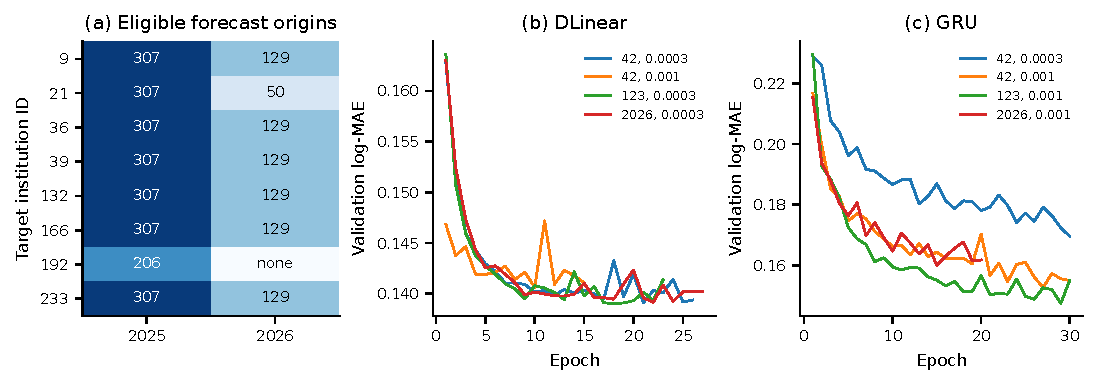
\includegraphics[width=\textwidth]{paper_coverage_learning.pdf}
\caption{Original availability and every neural seed/learning-rate validation trace. An absent eligible cell is not zero traffic. Hyperparameter selection uses validation institutions; repeated and overlapping histories do not create independent institutional replications.}\label{fig:coverage}
\end{figure*}

The new cohort selects eight institutions per original 2024 volume stratum using SHA-256 of \texttt{xai-replication-32-20261106-v1:\{id\}}. Its 217-candidate unused pool excludes all original-study and earlier development institutions. Hungarian matching uses log1p median GB and log1p(std/median), scaled by source descriptor standard deviations within stratum (constant dimension scale one). Matching distances, unavailable cells and undefined scores are retained without replacements.

Main timestamp plans have 2,016 source/target histories per fit over 63 new pair-years; the nested dense plan has 8,064 histories per GRU seed. Dense evaluation adds 6,048 histories per seed and reuses 72,576 main operator/seed records across three seeds exactly. Independent added-case queries agree with stored quality scores. The original bootstrap uses random seed 20261105; new pair-only and synchronized-calendar sensitivities use 20261106, all with 2,000 attempted draws. Every endpoint, including both horizons' dense uncertainty families, is preserved in \texttt{SENSITIVITY\_RESULTS.json} in the new-cohort artifact.

The local freeze followed the original outcome but preceded new-target scoring. It is not external preregistration. Source models/anchors and ISP overlap; original and new contrasts must remain separate. Historical manifests retain their unscored-at-freeze fields; completion records describe execution. Dataset credit: Josef Koumar, Karel Hynek, Kamil Je\v{r}\'abek and Pavel \v{S}i\v{s}ka, CESNET-TimeSeries26 (2026), \url{https://doi.org/10.5281/zenodo.21945629}, CC BY 4.0. Official observed values remain unchanged; selected files add native-grid coverage/artifact fields and compression.

\section{Original forecast distribution and calibration}
Table~\ref{tab:forecast} reports means across available target institution-year cells after averaging neural seeds. MASE uses each institution's observed eligible 2024 weekly absolute-difference scale, floored at $10^{-9}$ GB. This historical scaling is not target-outcome fitting. Raw MAE mixes institutions of different volumes; MASE supports within-institution scale comparisons. The table has 15 cells rather than a balanced 16-cell panel, so institutions with two available years receive two entries.

\begin{table}[t]\centering\caption{Frozen target forecasts. MAE in GB; available institution-year macro means, neural seeds averaged first. No model-ranking significance claim.}\label{tab:forecast}
\begin{tabular}{lrrrr}\toprule
&\multicolumn{2}{c}{1-hour endpoint}&\multicolumn{2}{c}{6-hour endpoint}\\
Model&MAE&MASE&MAE&MASE\\\midrule
Persistence&0.501&0.737&1.053&1.451\\
Daily&0.778&1.083&0.735&1.112\\
Weekly&0.654&1.075&0.643&1.053\\
Ridge&0.468&0.681&0.501&0.813\\
DLinear&0.471&0.682&0.503&0.812\\
GRU&0.470&0.684&0.607&0.909\\\bottomrule
\end{tabular}\end{table}

\begin{figure*}[t]\centering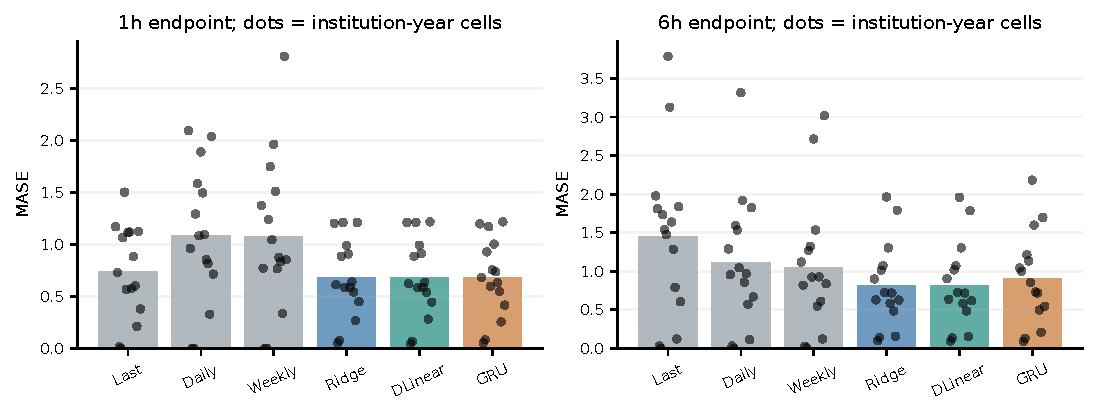
\includegraphics[width=\textwidth]{paper_forecast.pdf}
\caption{Frozen target forecasting. Bar heights are equal available institution-year macro MASE, after neural-seed averaging; black dots show the 15 underlying institution-year cells. Lower is better. The dispersion is descriptive; neither dots nor repeated training seeds are treated as independent network replications or model-ranking significance tests.}\label{fig:forecast}
\end{figure*}

Ridge, DLinear, and GRU are close at one hour. Figure~\ref{fig:forecast} shows that this similar average coexists with substantial institution-year heterogeneity. At six hours, Ridge and DLinear have lower descriptive MASE than GRU. These data do not support increasing model complexity solely for accuracy in this setup. Bias calibration changes one-hour MASE to 0.673, 0.676, and 0.683 for Ridge, DLinear, and GRU, respectively; their six-hour values become 0.818, 0.818, and 0.905. Calibration is not uniformly beneficial across horizons. We make no inferential claim about these small changes.

\section{Original pair/operator components and leave-one-pair-out diagnostic}
The primary comparison contains 369 paired origin/operator records before the complete-pair restriction. Seven pairs support both operators in both years. Their equally weighted mean source $Q$ is 0.7006 and target $Q$ is 0.6817, giving a target-minus-source contrast of $-0.0189$. The nominal 95\% interval is $[-0.0891,0.0533]$ from 1,853 valid bootstrap draws out of 2,000. This interval includes zero and changes of either sign. A lack of a detected decrease is not an equivalence or non-inferiority result: no equivalence margin was prespecified.

\begin{figure*}[t]\centering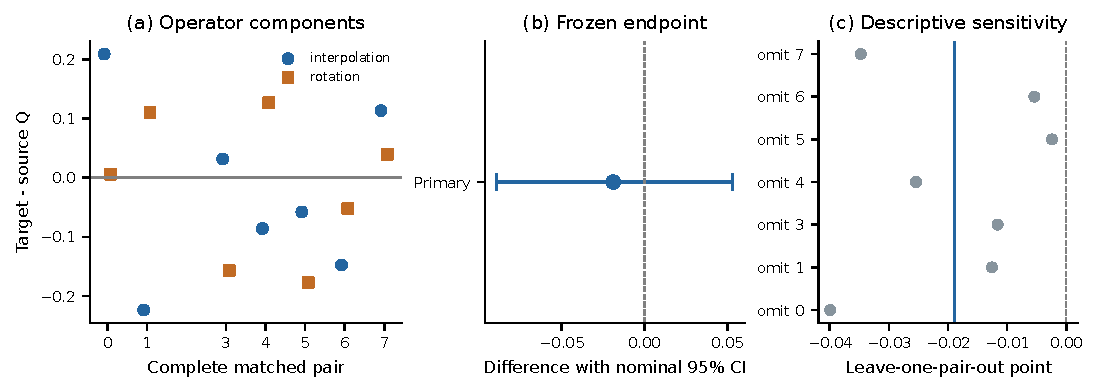
\includegraphics[width=\textwidth]{paper_primary_sensitivity.pdf}
\caption{Primary setting. (a) Complete-pair operator components, with the two years weighted equally; pair 2 is excluded. (b) The frozen primary contrast and its nominal 95\% interval. (c) Post-hoc leave-one-pair-out point estimates; these are descriptive sensitivity checks, not seven extra hypothesis tests or confidence intervals.}\label{fig:pairs}
\end{figure*}

Figure~\ref{fig:pairs} illustrates why aggregation needs care. Pair 0 has an interpolation contrast of $+0.209$ but a rotation contrast near $+0.006$; pair 1 has $-0.224$ and $+0.110$, respectively. This is evidence of dependence on the selected controlled operator. It is not evidence that either operator reveals true institutional causes. A post-hoc leave-one-pair-out diagnostic ranges from $-0.0399$ to $-0.0024$. All seven omitted-pair point estimates remain negative, but their movement relative to the small pooled contrast shows that the magnitude depends on a small panel. This diagnostic does not narrow the original interval, establish equivalence, or rescue an inconclusive primary finding.

\section{Original secondary reference contrasts}
\begin{figure*}[t]\centering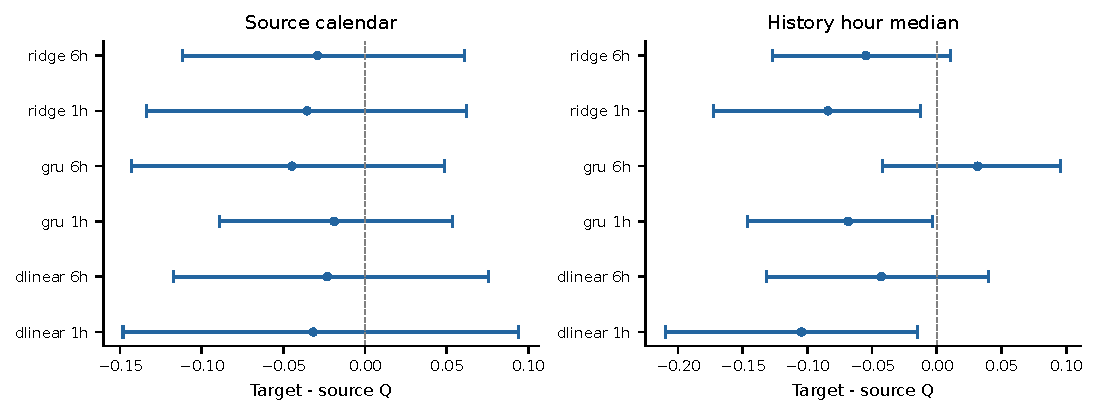
\includegraphics[width=\textwidth]{paper_secondary_forest.pdf}
\caption{All twelve frozen Shapley secondary model/horizon/reference contrasts. Seven complete pairs; nominal paired bootstrap 95\% intervals with no multiplicity adjustment. Source-calendar GRU h1 is the prespecified primary setting; a stronger-looking alternate reference is not promoted after observing the targets.}\label{fig:secondary}
\end{figure*}
The source-calendar one-hour intervals include zero for all three models. Under the history-hour-median reference, the three nominal intervals fall below zero (Fig.~\ref{fig:secondary}). These are exploratory results, and the references explain distinct prediction contrasts. They do not justify replacing the primary hypothesis after observing results or declaring the median reference defective. Six-hour contrasts also vary: the GRU history-median estimate is positive ($+0.031$), with an interval spanning zero. The twelve-cell table is supplied in the artifact and visualized in Fig.~\ref{fig:secondary}.

\section{Original numerical and denominator audit}
Exact Shapley efficiency residuals are at most $3.56\cdot10^{-15}$ GB. Independent enumeration of all permutations on sampled Ridge, DLinear, and GRU cases agrees with the subset formula. This confirms the implemented finite game arithmetic on the audited cases; it does not validate the scientific semantics of the reference.

\begin{table}[t]\centering\caption{IG numerical acceptance across both references and horizons, frozen arm only. Cases include source/target and neural seed replicates. Failures remain recorded.}\label{tab:ig}
\begin{tabular}{lrrr}\toprule Model&Cases&Accepted&Failed\\\midrule
Ridge&480&450&30\\
DLinear&1,440&1,335&105\\
GRU&1,440&1,365&75\\\midrule
Total&3,360&3,150&210\\\bottomrule\end{tabular}\end{table}
IG passes the fixed checks in 93.75\% of cases (Table~\ref{tab:ig}). Failures can occur even for log-space Ridge because the attributed GB function contains nonlinear transformations and a clipping boundary. We did not relax tolerances or increase the quadrature limit after evaluating targets. These failures establish numerical non-acceptance under this procedure, not theoretical invalidity of IG. Comparisons of IG rankings require common accepted cases; we avoid an all-case superiority claim from its smaller subset.

Across non-IG methods, each has 53,760 operator-score records, of which 51,944 are defined. The 1,816 non-discriminating records per method have insufficient oracle--random separation. Of 6,720 IG operator records, 6,137 are scored after numerical and denominator screening. Figure~\ref{fig:ig} further disaggregates numerical acceptance by reference and horizon; pooled rejection alone hides these differences.

\begin{figure}[t]\centering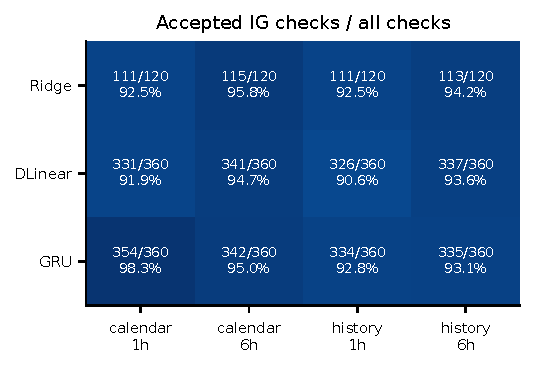
\includegraphics[width=\columnwidth]{paper_ig_audit.pdf}
\caption{Accepted IG numerical checks by model, reference and endpoint. Numerators and denominators include repeated neural seeds; they are numerical workloads, not independent subjects. ``Calendar'' and ``history'' denote the two attribution references.}\label{fig:ig}
\end{figure}

These records are repeated model/reference/horizon/operator evaluations, not independent samples. Final paired averages additionally require complete neural seeds and timestamp-matched source and target scores. Consequently, neither 168,000 total records nor 3,360 IG checks should be presented as the inferential sample size.

\section{Original common accepted Shapley/IG cases}
A matched visualization compares Shapley and IG only where both have a defined $Q$ on the same history/reference/operator, and all three GRU seeds meet these requirements. For frozen GRU h1 with the source-calendar reference, this leaves 627 operator/seed records, or 209 history/operator units after seed averaging, across 29 available institution-year cells from the matched source and target institutions. We then average within institution-year for display.

\begin{figure}[t]\centering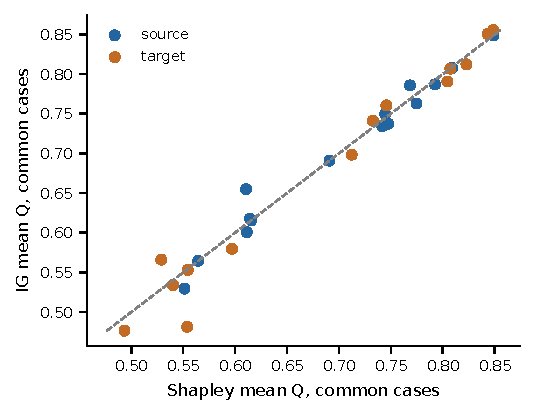
\includegraphics[width=\columnwidth]{paper_common_cases.pdf}
\caption{Exploratory common-case comparison of frozen GRU h1 source-calendar Shapley and IG. Each point is one available institution-year mean after requiring all three valid seeds and averaging only shared history/operator cases. The diagonal marks equal $Q$. Agreement on this screened subset does not establish universal superiority or explain rejected cases.}\label{fig:common}
\end{figure}

Most displayed means are close to the equality line (Fig.~\ref{fig:common}), although individual cells differ. This restricted subset is not interchangeable with the all-case primary endpoint: numerical acceptance and oracle-gap screening can change the population being summarized. No new inferential superiority claim is made from the plot.

\section{Computational workload and independent rerun}
A full notebook reproduction on an Apple M5 laptop with 16 GB RAM and four CPU threads completed in 529.5 seconds. Training consumed 324.3 seconds, forecast evaluation 9.7 seconds, attribution evaluation 184.7 seconds, and the remaining 10.8 seconds covered notebook diagnostics, analysis and overhead. These figures describe this implementation on this machine, not a hardware benchmark or a projected cloud runtime.

The short runtime has concrete causes. DLinear has 676 trainable parameters and GRU 3,426; Ridge has 338 fitted coefficients/intercepts across its two heads. Each neural epoch samples 32,768 windows, rather than making a full pass through all 227,478 eligible source windows. Across eight seed/learning-rate training fits, 201 executed epochs produce 6,586,368 sampled window exposures, including repetitions. This is computational exposure, not 6.59 million independent observations.

Attribution is also deliberately coarse and sampled: seven day groups require only 128 coalition evaluations per game, and the 5,040 ordering utilities are looked up from cached coalition responses. They are not 5,040 independent neural forward passes per explanation. The full attribution audit uses 480 histories per fitted model, with IG restricted to 120. Thus a fast run is compatible with complete execution of this specified benchmark; it does not establish that a broader benchmark has been exhausted.

Every code cell in the full-run notebook completed without error. All six neural parameter state dictionaries reproduced exactly; binary checkpoint hashes differ because metadata includes newly measured training runtimes. The primary point, interval and valid-draw count reproduced exactly. A separate audit rechecked data/code hashes, all saved forecast metrics, representative checkpoint and attribution queries, and the primary point. Reproduction strengthens confidence in implementation consistency; it does not provide new independent institutions or an untouched test set.


\section{Local forecast and attribution example}
The example uses original-cohort institution 132 at its earliest selected 2025 origin, 15 April 00:00 UTC, frozen GRU seed 42. Selection uses metadata, not forecast accuracy. The h1 forecast is 0.322 GB versus observed 0.00665 GB; h6 is 1.479 versus 0.184 GB. Both reference-specific IG allocations pass at 64 nodes. Exact allocation and accepted integration do not imply a successful forecast or causal demand explanation.
\begin{figure*}[t]\centering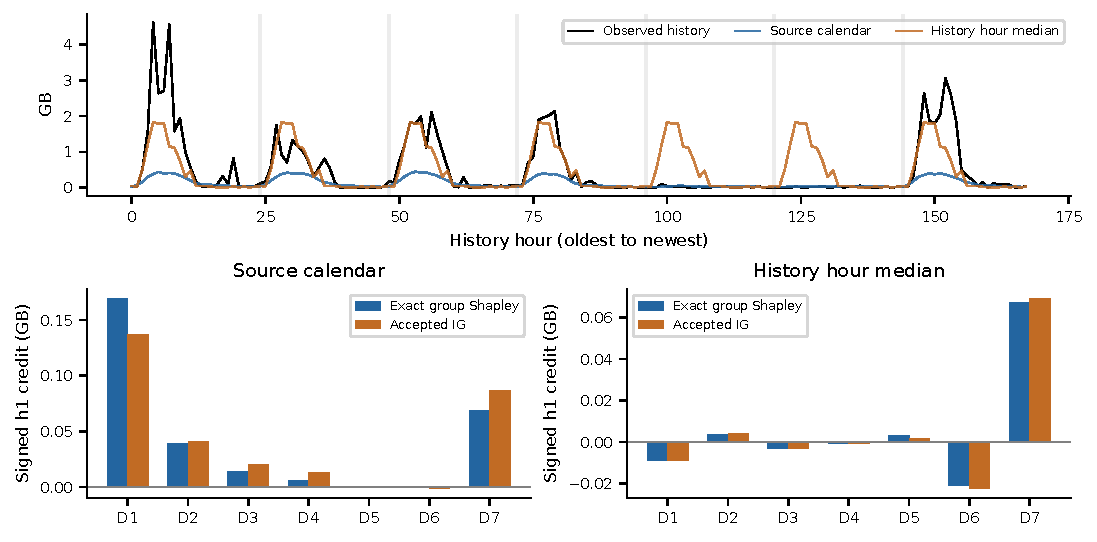
\includegraphics[width=\textwidth]{paper_local_case.pdf}
\caption{Metadata-selected original-cohort example: institution 132, 15 April 2025, frozen GRU seed 42. Top: history and references. Bottom: signed h1 daily Shapley/accepted-IG allocations, oldest day first. Numerical acceptance and exact allocation do not imply forecast success or causal demand attribution.}\label{fig:supplocal}
\end{figure*}

\section{Focused post-hoc checks: additional counts}
The conference-check plan and seven code/selection files were locally frozen after original/new-cohort outcomes were known and before randomized-model outcomes. Original scientific freezes remain unchanged. Panel A common-case comparison uses 1,813 source and 1,824 target history/operator cases, 61 institution-years and 31 institutions per cohort. Panel B has 451 source and 452 target common cases before the complete-operator cell requirement; the latter removes one target case, giving 451 used cases in each cohort and 61/60 institution-years. Every compared method must have all three defined seeds; IG additionally passes its numerical checks.

For the parameter control, each stage contains 567 records per cohort, combining 63 histories, three trained seeds and three randomization replicates. Trained Shapley vectors are nonflat for all selected seed/history records. Randomized nonflat counts are 425/342 (head/head+GRU) for sources and 439/367 for targets. The two-stage common panel contains 337 source and 364 target records and at least one comparable record for each of the 126 histories. Actual randomized predictions are clipped in 203/225 source and 167/201 target records; prediction clipping and a flat allocation vector are different conditions.

Replicate keys are 701, 1701 and 2701. Head RNG seed is trained seed times 10,000 plus the key; GRU reset adds 100,000,000. Learned layers use their standard reset initialization in double precision. The same randomized head is retained across cumulative stages; source buffers and the architecture's fixed residual route are unchanged. Signed-pattern distance is one half of the L1 difference between signed allocations normalized by their L1 norms, defined only when each norm exceeds $10^{-9}$ GB. Spearman correlation uses the seven absolute daily allocations and is undefined for constant vectors. Coverage and complete raw records remain available, without a post-outcome threshold adjustment or extra replicates.

Independent audits reproduce common-case macro means within $1.12\cdot10^{-16}$, normalized-pattern distances exactly, and sampled randomized-checkpoint predictions/allocations exactly. A full-permutation Shapley check agrees on the audited randomized cases. Copied-model differences are zero. The control takes approximately 40 seconds on the local CPU with no training; this is computational workload, not new independent deployment evidence. The added plot-style helper changes only visual placement of the legend after computation; the frozen analysis code and numerical outputs remain unchanged.

\end{document}
